%%%%%%%%%%%%%%%%%%%%%%%%%%%%%%%%%%%%%%%%%
% The Legrand Orange Book
% LaTeX Template
% Version 1.3 (21/8/13)
%
% This template has been downloaded from:
% http://www.LaTeXTemplates.com
%
% Original author:
% Mathias Legrand (legrand.mathias@gmail.com)
%
% License:
% CC BY-NC-SA 3.0 (http://creativecommons.org/licenses/by-nc-sa/3.0/)
%
% Compiling this template:
% This template uses biber for its bibliography and makeindex for its index.
% When you first open the template, compile it from the command line with the 
% commands below to make sure your LaTeX distribution is configured correctly:
%
% 1) pdflatex main
% 2) makeindex main.idx -s StyleInd.ist
% 3) biber main
% 4) pdflatex main x 2
%
% After this, when you wish to update the bibliography/index use the appropriate
% command above and make sure to compile with pdflatex several times 
% afterwards to propagate your changes to the document.
%
% This template also uses a number of packages which may need to be
% updated to the newest versions for the template to compile. It is strongly
% recommended you update your LaTeX distribution if you have any
% compilation errors.
%
% Important note:
% Chapter heading images should have a 2:1 width:height ratio,
% e.g. 920px width and 460px height.
%
%%%%%%%%%%%%%%%%%%%%%%%%%%%%%%%%%%%%%%%%%

%----------------------------------------------------------------------------------------
%	PACKAGES AND OTHER DOCUMENT CONFIGURATIONS
%----------------------------------------------------------------------------------------

\documentclass[11pt,fleqn]{book} % Default font size and left-justified equations

\usepackage[top=3cm,bottom=3cm,left=3.2cm,right=3.2cm,headsep=10pt,a4paper]{geometry} % Page margins

\usepackage{xcolor} % Required for specifying colors by name
\definecolor{ocre}{RGB}{243,102,25} % Define the orange color used for highlighting throughout the book

% Font Settings
\usepackage{avant} % Use the Avantgarde font for headings
%\usepackage{times} % Use the Times font for headings
\usepackage{mathptmx} % Use the Adobe Times Roman as the default text font together with math symbols from the Sym­bol, Chancery and Com­puter Modern fonts

\usepackage{microtype} % Slightly tweak font spacing for aesthetics
\usepackage[utf8]{inputenc} % Required for including letters with accents
\usepackage[T1]{fontenc} % Use 8-bit encoding that has 256 glyphs

\usepackage{color}
\usepackage{listings}
\usepackage{float}


\usepackage{amsmath}
\usepackage{hyperref} % references  as links

\usepackage{multicol}
% Bibliography
%\usepackage[style=alphabetic,sorting=nyt,sortcites=true,autopunct=true,babel=hyphen,hyperref=true,abbreviate=false,backref=true,backend=biber]{biblatex}
%\addbibresource{bibliography.bib} % BibTeX bibliography file
%\defbibheading{bibempty}{}00

% Index
\usepackage{calc} % For simpler calculation - used for spacing the index letter headings correctly
\usepackage{makeidx} % Required to make an index
\makeindex % Tells LaTeX to create the files required for indexing

%----------------------------------------------------------------------------------------

%----------------------------------------------------------------------------------------
%	VARIOUS REQUIRED PACKAGES
%----------------------------------------------------------------------------------------

\usepackage{titlesec} % Allows customization of titles

\usepackage{graphicx} % Required for including pictures
\graphicspath{{Pictures/}} % Specifies the directory where pictures are stored

\usepackage{lipsum} % Inserts dummy text

\usepackage{tikz} % Required for drawing custom shapes

\usepackage[english]{babel} % English language/hyphenation

\usepackage{enumitem} % Customize lists
\setlist{nolistsep} % Reduce spacing between bullet points and numbered lists

\usepackage{booktabs} % Required for nicer horizontal rules in tables

\usepackage{eso-pic} % Required for specifying an image background in the title page

%----------------------------------------------------------------------------------------
%	MAIN TABLE OF CONTENTS
%----------------------------------------------------------------------------------------

\usepackage{titletoc} % Required for manipulating the table of contents

\contentsmargin{0cm} % Removes the default margin
% Chapter text styling
\titlecontents{chapter}[1.25cm] % Indentation
{\addvspace{15pt}\large\sffamily\bfseries} % Spacing and font options for chapters
{\color{ocre!60}\contentslabel[\Large\thecontentslabel]{1.25cm}\color{ocre}} % Chapter number
{}  
{\color{ocre!60}\normalsize\sffamily\bfseries\;\titlerule*[.5pc]{.}\;\thecontentspage} % Page number
% Section text styling
\titlecontents{section}[1.25cm] % Indentation
{\addvspace{5pt}\sffamily\bfseries} % Spacing and font options for sections
{\contentslabel[\thecontentslabel]{1.25cm}} % Section number
{}
{\sffamily\hfill\color{black}\thecontentspage} % Page number
[]
% Subsection text styling
\titlecontents{subsection}[1.25cm] % Indentation
{\addvspace{1pt}\sffamily\small} % Spacing and font options for subsections
{\contentslabel[\thecontentslabel]{1.25cm}} % Subsection number
{}
{\sffamily\;\titlerule*[.5pc]{.}\;\thecontentspage} % Page number
[] 

%----------------------------------------------------------------------------------------
%	MINI TABLE OF CONTENTS IN CHAPTER HEADS
%----------------------------------------------------------------------------------------

% Section text styling
\titlecontents{lsection}[0em] % Indendating
{\footnotesize\sffamily} % Font settings
{}
{}
{}

% Subsection text styling
\titlecontents{lsubsection}[.5em] % Indentation
{\normalfont\footnotesize\sffamily} % Font settings
{}
{}
{}
 
%----------------------------------------------------------------------------------------
%	PAGE HEADERS
%----------------------------------------------------------------------------------------

\usepackage{fancyhdr} % Required for header and footer configuration

\pagestyle{fancy}
\renewcommand{\chaptermark}[1]{\markboth{\sffamily\normalsize\bfseries #1}{}} % Chapter text font settings
\renewcommand{\sectionmark}[1]{\markright{\sffamily\normalsize\thesection\hspace{5pt}#1}{}} % Section text font settings
\fancyhf{} \fancyhead[LE,RO]{\sffamily\normalsize\thepage} % Font setting for the page number in the header
\fancyhead[LO]{\rightmark} % Print the nearest section name on the left side of odd pages
\fancyhead[RE]{\leftmark} % Print the current chapter name on the right side of even pages
\renewcommand{\headrulewidth}{0.5pt} % Width of the rule under the header
\addtolength{\headheight}{2.5pt} % Increase the spacing around the header slightly
\renewcommand{\footrulewidth}{0pt} % Removes the rule in the footer
\fancypagestyle{plain}{\fancyhead{}\renewcommand{\headrulewidth}{0pt}} % Style for when a plain pagestyle is specified

% Removes the header from odd empty pages at the end of chapters
\makeatletter
\renewcommand{\cleardoublepage}{
\clearpage\ifodd\c@page\else
\hbox{}
\vspace*{\fill}
\thispagestyle{empty}
\newpage
\fi}

%----------------------------------------------------------------------------------------
%	THEOREM STYLES
%----------------------------------------------------------------------------------------

\usepackage{amsmath,amsfonts,amssymb,amsthm} % For including math equations, theorems, symbols, etc

\newcommand{\intoo}[2]{\mathopen{]}#1\,;#2\mathclose{[}}
\newcommand{\ud}{\mathop{\mathrm{{}d}}\mathopen{}}
\newcommand{\intff}[2]{\mathopen{[}#1\,;#2\mathclose{]}}
\newtheorem{notation}{Notation}[chapter]

%%%%%%%%%%%%%%%%%%%%%%%%%%%%%%%%%%%%%%%%%%%%%%%%%%%%%%%%%%%%%%%%%%%%%%%%%%%
%%%%%%%%%%%%%%%%%%%% dedicated to boxed/framed environements %%%%%%%%%%%%%%
%%%%%%%%%%%%%%%%%%%%%%%%%%%%%%%%%%%%%%%%%%%%%%%%%%%%%%%%%%%%%%%%%%%%%%%%%%%
\newtheoremstyle{ocrenumbox}% % Theorem style name
{0pt}% Space above
{0pt}% Space below
{\normalfont}% % Body font
{}% Indent amount
{\small\bf\sffamily\color{ocre}}% % Theorem head font
{\;}% Punctuation after theorem head
{0.25em}% Space after theorem head
{\small\sffamily\color{ocre}\thmname{#1}\nobreakspace\thmnumber{\@ifnotempty{#1}{}\@upn{#2}}% Theorem text (e.g. Theorem 2.1)
\thmnote{\nobreakspace\the\thm@notefont\sffamily\bfseries\color{black}---\nobreakspace#3.}} % Optional theorem note
\renewcommand{\qedsymbol}{$\blacksquare$}% Optional qed square

\newtheoremstyle{blacknumex}% Theorem style name
{5pt}% Space above
{5pt}% Space below
{\normalfont}% Body font
{} % Indent amount
{\small\bf\sffamily}% Theorem head font
{\;}% Punctuation after theorem head
{0.25em}% Space after theorem head
{\small\sffamily{\tiny\ensuremath{\blacksquare}}\nobreakspace\thmname{#1}\nobreakspace\thmnumber{\@ifnotempty{#1}{}\@upn{#2}}% Theorem text (e.g. Theorem 2.1)
\thmnote{\nobreakspace\the\thm@notefont\sffamily\bfseries---\nobreakspace#3.}}% Optional theorem note

\newtheoremstyle{blacknumbox} % Theorem style name
{0pt}% Space above
{0pt}% Space below
{\normalfont}% Body font
{}% Indent amount
{\small\bf\sffamily}% Theorem head font
{\;}% Punctuation after theorem head
{\newline}% Space after theorem head
{\small\sffamily\thmname{#1}\nobreakspace\thmnumber{\@ifnotempty{#1}{}\@upn{#2}}% Theorem text (e.g. Theorem 2.1)
\thmnote{\nobreakspace\the\thm@notefont\sffamily\bfseries---\nobreakspace#3:}}% Optional theorem note

%%%%%%%%%%%%%%%%%%%%%%%%%%%%%%%%%%%%%%%%%%%%%%%%%%%%%%%%%%%%%%%%%%%%%%%%%%%
%%%%%%%%%%%%% dedicated to non-boxed/non-framed environements %%%%%%%%%%%%%
%%%%%%%%%%%%%%%%%%%%%%%%%%%%%%%%%%%%%%%%%%%%%%%%%%%%%%%%%%%%%%%%%%%%%%%%%%%
\newtheoremstyle{ocrenum}% % Theorem style name
{5pt}% Space above
{5pt}% Space below
{\normalfont}% % Body font
{}% Indent amount
{\small\bf\sffamily\color{ocre}}% % Theorem head font
{\;}% Punctuation after theorem head
{0.25em}% Space after theorem head
{\small\sffamily\color{ocre}\thmname{#1}\nobreakspace\thmnumber{\@ifnotempty{#1}{}\@upn{#2}}% Theorem text (e.g. Theorem 2.1)
\thmnote{\nobreakspace\the\thm@notefont\sffamily\bfseries\color{black}---\nobreakspace#3.}} % Optional theorem note
\renewcommand{\qedsymbol}{$\blacksquare$}% Optional qed square
\makeatother

% Defines the theorem text style for each type of theorem to one of the three styles above
\newcounter{dummy} 
\numberwithin{dummy}{section}
\theoremstyle{ocrenumbox}
\newtheorem{theoremeT}[dummy]{Theorem}
\newtheorem{problem}{Problem}[chapter]
\newtheorem{exerciseT}{Zadanie}[chapter]
\theoremstyle{blacknumex}
\newtheorem{exampleT}{Example}[chapter]
\theoremstyle{blacknumbox}
\newtheorem{vocabulary}{Vocabulary}[chapter]
\newtheorem{definitionT}{Definition}[section]
\newtheorem{corollaryT}[dummy]{Kod}
\theoremstyle{ocrenum}
\newtheorem{proposition}[dummy]{Proposition}

%----------------------------------------------------------------------------------------
%	DEFINITION OF COLORED BOXES
%----------------------------------------------------------------------------------------

\RequirePackage[framemethod=default]{mdframed} % Required for creating the theorem, definition, exercise and corollary boxes

% Theorem box
\newmdenv[skipabove=7pt,
skipbelow=7pt,
backgroundcolor=black!5,
linecolor=ocre,
innerleftmargin=5pt,
innerrightmargin=5pt,
innertopmargin=5pt,
leftmargin=0cm,
rightmargin=0cm,
innerbottommargin=5pt]{tBox}

% Exercise box	  
\newmdenv[skipabove=7pt,
skipbelow=7pt,
rightline=false,
leftline=true,
topline=false,
bottomline=false,
backgroundcolor=ocre!10,
linecolor=ocre,
innerleftmargin=5pt,
innerrightmargin=5pt,
innertopmargin=5pt,
innerbottommargin=5pt,
leftmargin=0cm,
rightmargin=0cm,
linewidth=4pt]{eBox}	

% Definition box
\newmdenv[skipabove=7pt,
skipbelow=7pt,
rightline=false,
leftline=true,
topline=false,
bottomline=false,
linecolor=ocre,
innerleftmargin=5pt,
innerrightmargin=5pt,
innertopmargin=0pt,
leftmargin=0cm,
rightmargin=0cm,
linewidth=4pt,
innerbottommargin=0pt]{dBox}	

% Corollary box
\newmdenv[skipabove=0pt,
skipbelow=7pt,
rightline=false,
leftline=true,
topline=false,
bottomline=false,
linecolor=gray,
backgroundcolor=black!5,
innerleftmargin=5pt,
innerrightmargin=5pt,
innertopmargin=5pt,
leftmargin=0cm,
rightmargin=0cm,
linewidth=4pt,
innerbottommargin=5pt]{cBox}				  
		  

% Creates an environment for each type of theorem and assigns it a theorem text style from the "Theorem Styles" section above and a colored box from above
\newenvironment{theorem}{\begin{tBox}\begin{theoremeT}}{\end{theoremeT}\end{tBox}}
\newenvironment{exercise}{\begin{eBox}\begin{exerciseT}}{\hfill{\color{ocre}\tiny\ensuremath{\blacksquare}}\end{exerciseT}\end{eBox}}				  
\newenvironment{definition}{\begin{dBox}\begin{definitionT}}{\end{definitionT}\end{dBox}}	
\newenvironment{example}{\begin{exampleT}}{\hfill{\tiny\ensuremath{\blacksquare}}\end{exampleT}}		
\newenvironment{corollary}{\begin{cBox}\begin{corollaryT}}{\end{corollaryT}\end{cBox}}	
%\newenvironment{corollary}{\begin{cBox}\end{cBox}}
%----------------------------------------------------------------------------------------
%	REMARK ENVIRONMENT
%----------------------------------------------------------------------------------------

\newenvironment{remark}{\par\vskip10pt\small % Vertical white space above the remark and smaller font size
\begin{list}{}{
\leftmargin=35pt % Indentation on the left
\rightmargin=25pt}\item\ignorespaces % Indentation on the right
\makebox[-2.5pt]{\begin{tikzpicture}[overlay]
\node[draw=ocre!60,line width=1pt,circle,fill=ocre!25,font=\sffamily\bfseries,inner sep=2pt,outer sep=0pt] at (-15pt,0pt){\textcolor{ocre}{R}};\end{tikzpicture}} % Orange R in a circle
\advance\baselineskip -1pt}{\end{list}\vskip5pt} % Tighter line spacing and white space after remark

%----------------------------------------------------------------------------------------
%	SECTION NUMBERING IN THE MARGIN
%----------------------------------------------------------------------------------------

\makeatletter
\renewcommand{\@seccntformat}[1]{\llap{\textcolor{ocre}{\csname the#1\endcsname}\hspace{1em}}}                    
\renewcommand{\section}{\@startsection{section}{1}{\z@}
{-4ex \@plus -1ex \@minus -.4ex}
{1ex \@plus.2ex }
{\normalfont\large\sffamily\bfseries}}
\renewcommand{\subsection}{\@startsection {subsection}{2}{\z@}
{-3ex \@plus -0.1ex \@minus -.4ex}
{0.5ex \@plus.2ex }
{\normalfont\sffamily\bfseries}}
\renewcommand{\subsubsection}{\@startsection {subsubsection}{3}{\z@}
{-2ex \@plus -0.1ex \@minus -.2ex}
{0.2ex \@plus.2ex }
{\normalfont\small\sffamily\bfseries}}                        
\renewcommand\paragraph{\@startsection{paragraph}{4}{\z@}
{-2ex \@plus-.2ex \@minus .2ex}
{0.1ex}
{\normalfont\small\sffamily\bfseries}}

%----------------------------------------------------------------------------------------
%	CHAPTER HEADINGS
%----------------------------------------------------------------------------------------

\newcommand{\thechapterimage}{}
\newcommand{\chapterimage}[1]{\renewcommand{\thechapterimage}{#1}}
\def\thechapter{\arabic{chapter}}
\def\@makechapterhead#1{
\thispagestyle{empty}
{\centering \normalfont\sffamily
\ifnum \c@secnumdepth >\m@ne
\if@mainmatter
\startcontents
\begin{tikzpicture}[remember picture,overlay]
\node at (current page.north west)
{\begin{tikzpicture}[remember picture,overlay]

\node[anchor=north west,inner sep=0pt] at (0,0) {\includegraphics[width=\paperwidth]{\thechapterimage}};

%Commenting the 3 lines below removes the small contents box in the chapter heading
%\draw[fill=white,opacity=.6] (1cm,0) rectangle (8cm,-7cm);
%\node[anchor=north west] at (1cm,.25cm) {\parbox[t][8cm][t]{6.5cm}{\huge\bfseries\flushleft \printcontents{l}{1}{\setcounter{tocdepth}{2}}}};

\draw[anchor=west] (2cm,-9cm) node [rounded corners=25pt,fill=white,fill opacity=.6,text opacity=1,draw=ocre,draw opacity=1,line width=2pt,inner sep=15pt]{\huge\sffamily\bfseries\textcolor{black}{\thechapter\ ---\ #1\vphantom{plPQq}\makebox[22cm]{}}};
\end{tikzpicture}};
\end{tikzpicture}}\par\vspace*{230\p@}
\fi
\fi
}
\def\@makeschapterhead#1{
\thispagestyle{empty}
{\centering \normalfont\sffamily
\ifnum \c@secnumdepth >\m@ne
\if@mainmatter
\startcontents
\begin{tikzpicture}[remember picture,overlay]
\node at (current page.north west)
{\begin{tikzpicture}[remember picture,overlay]
\node[anchor=north west] at (-4pt,4pt) {\includegraphics[width=\paperwidth]{\thechapterimage}};
\draw[anchor=west] (5cm,-9cm) node [rounded corners=25pt,fill=white,opacity=.7,inner sep=15.5pt]{\huge\sffamily\bfseries\textcolor{black}{\vphantom{plPQq}\makebox[22cm]{}}};
\draw[anchor=west] (5cm,-9cm) node [rounded corners=25pt,draw=ocre,line width=2pt,inner sep=15pt]{\huge\sffamily\bfseries\textcolor{black}{#1\vphantom{plPQq}\makebox[22cm]{}}};
\end{tikzpicture}};
\end{tikzpicture}}\par\vspace*{230\p@}
\fi
\fi
}
\makeatother % Insert the commands.tex file which contains the majority of the structure behind the template

\lstset{language=Verilog}          % Set your language (you can change the language for each code-block optionally)
\lstset{breaklines=true}

\definecolor{mygreen}{rgb}{0,0.6,0}

\lstset{ %
  %basicstyle=\footnotesize,
  %commentstyle=\color{mygreen},    % comment style
  deletekeywords={...},            % if you want to delete keywords from the given language
  %frame=single,                    % adds a frame around the code
  keepspaces=true,                 % keeps spaces in text, useful for keeping indentation of code (possibly needs columns=flexible)
  %keywordstyle=\color{blue},       % keyword style
  language=Verilog,                  % the language of the code
  basicstyle=\footnotesize\ttfamily,
  %keywordstyle=\bfseries\color{black},
  commentstyle=\color{gray},
  identifierstyle=\color{blue},
  stringstyle=\color{orange}
}
\renewcommand{\ttdefault}{pcr}
\begin{document}

%----------------------------------------------------------------------------------------
%	TITLE PAGE
%----------------------------------------------------------------------------------------

\begingroup
\thispagestyle{empty}
\AddToShipoutPicture*{\put(6,5){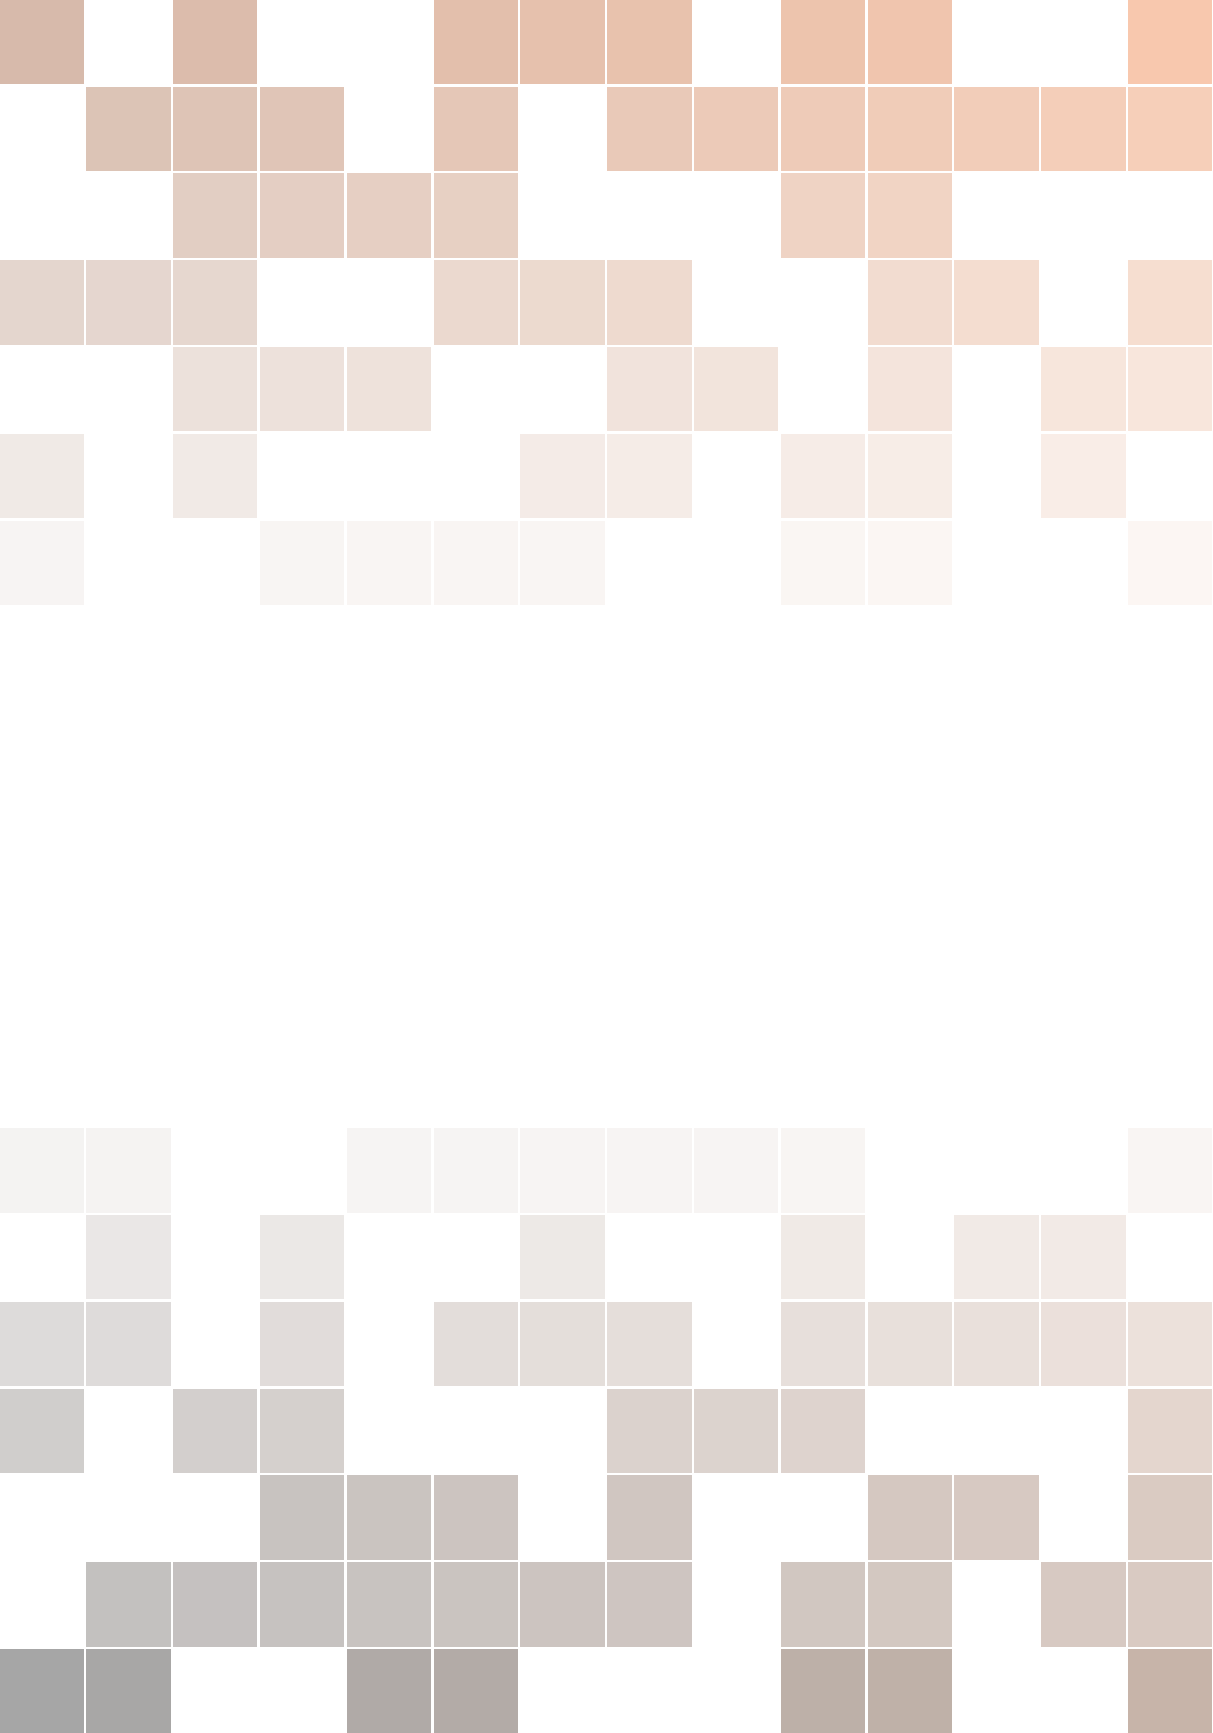
\includegraphics[scale=1]{images/background.pdf}}} % Image background
\centering
\vspace*{8cm}
\par\normalfont\fontsize{35}{35}\sffamily\selectfont
%Programowo-sprzętowa realizacja algorytmów\par % Book title
Detekcja koloru skóry z wykorzystaniem sieci neuronowych.\par % Book title
\vspace*{1cm}
{\fontsize{23}{23}\Huge Krzysztof Odrzywołek, \\ Michał Pietruszka, Rafał Włodarz}\par % Author name
\endgroup

%----------------------------------------------------------------------------------------
%	COPYRIGHT PAGE
%----------------------------------------------------------------------------------------

\newpage
~\vfill
\thispagestyle{empty}

\noindent Copyright \copyright\ 2015 \\  Krzysztof Odrzywołek, Michał Pietruszka, Rafał Włodarz\\ % Copyright notice

\noindent \textsc{Published by AGH}\\ % Publisher

%\noindent \textsc{book-website.com}\\ % URL

%\noindent Licensed under the Creative Commons Attribution-NonCommercial 3.0 Unported License (the ``License''). You may not use this file except in compliance with the License. You may obtain a copy of the License at \url{http://creativecommons.org/licenses/by-nc/3.0}. Unless required by applicable law or agreed to in writing, software distributed under the License is distributed on an \textsc{``AS IS'' BASIS, WITHOUT WARRANTIES OR CONDITIONS OF ANY KIND}, either express or implied. See the License for the specific language governing permissions and limitations under the License.\\ % License information

\noindent \textit{First printing, January 2015} % Printing/edition date

%----------------------------------------------------------------------------------------
%	TABLE OF CONTENTS
%----------------------------------------------------------------------------------------

\chapterimage{images/chapter_head_1.pdf} % Table of contents heading image

\pagestyle{empty} % No headers

\tableofcontents % Print the table of contents itself

\cleardoublepage % Forces the first chapter to start on an odd page so it's on the right

\pagestyle{fancy} % Print headers again

%----------------------------------------------------------------------------------------
%	CHAPTERS
%----------------------------------------------------------------------------------------
\chapter{Wstep}
\label{cha:introduction}

\section{Opis projektu}
Celem projektu było zrealizowanie algorytmu opartego na sieciach neuronowych którego zadaniem było rozpoznawanie skóry na podstawie obrazu z kamery w czasie rzeczywistym. 



\chapter{Realizacja projektu}
\label{cha:realizacja}

Realizacja projektu została podzielony na kilka etapów w których każdy jest zależna od  poprzedniego. Najważniejszymi etapami są: teoretyczne przygotowanie do zagadnienia wraz z doborem topologii sieci, implementacja algorytmu w środowisku MATLAB wraz z algorytmem uczenia sieci oraz ostateczna jego realizacja na układzie fpga. 
\section{Dobór topologii sieci}

Wybór odpowiedniej topologii sieci wymagał znajomości teoretycznej zagadnień związanych z algorytmami opartymi na sieciach neuronowych, wykorzystania własnego doświadczenia związanego z tymi zagadnieniami oraz realizacją algorytmów na układach fpga. Ze względu na niewystarczającą wiedzę w temacie sieci neuronowych, początkowa faza projektu opierała się na poszukiwaniu informacji o zagadnieniach zbliżonych do tematu projektu. Okazało się, iż bardzo zbliżony projekt został już zrealizowany i opisany w \cite{fdciuss}. Artykuł przedstawia dokładne etapy realizacji projektu którego celem było rozpoznawanie twarzy. Zawierał on również dokładny opis topologi sieci oraz sposób przygotowania danych do przetwarzania. 

Informacje te okazały się bardzo pomocne, pozwoliły one rozpocząć doświadczalny dobór topologi sieci, która pozwoli na poprawne przetwarzanie danych wejściowych. 
Podstawą do przeprowadzania takich eksperymentów było zdobycie bazy (została ona załączona wraz z plikami projektu), która umożliwi naukę sieci. Baza posiada zbiór danych przygotowany w formie 4 wartości odpowiadających poszczególnym wartością RGB oraz oczekiwanemu wyjściu z sieci, którego wartości zamykają się w zbiorze {0,1}. Świadczy ono o tym czy na podstawie określonego wejścia powinna zostać wykryta skóra.

Liczna baza danych wypełniona takimi rekordami pozwoliła na przeprowadzanie pierwszych doświadczeń. Na podstawie zdobytych informacji dowiedzieliśmy się, iż jakość wykrywania pikseli przedstawiających skórę znacznie wzrasta jeśli na wejście sieci oprócz sygnałów RGB podawane zostaną również CbCr(wartości sygnałów z modelu przestrzeni kolorów YCbCr) oraz HS(wartości sygnałów z przestrzeni barw HSV). Aby otrzymać pełny wektor danych wejściowych zaimplementowano algorytm w postaci skryptu w programie MATLAB, który na podstawie wartości RGB wyznaczał pozostałe parametry. Tak przygotowane dane wejściowe podawano na wejście wbudowanej sieci neuronowej w środowisko MATLAB, a następnie na podstawie przykładowego zdjęcia określano czy sieć poprawnie rozpoznaje skórę na przedstawionym obrazie. Ze względu na łatwą konfigurację topologii sieci sposób ten okazał umożliwił szybkie przetestowanie wielu wariantów oraz wybranie najlepszego w interesującym nas zakresie.

\begin{figure}[tbph!]
	\centering
	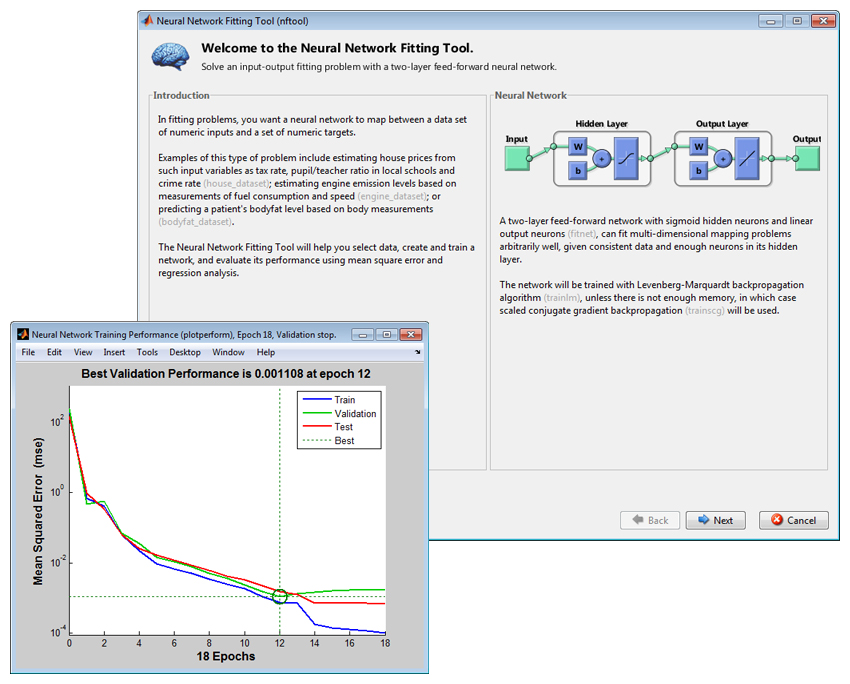
\includegraphics[width=0.9\linewidth]{images/matlabnn.jpg}
	\caption{Narzędzie środowiska MATLAB służące do testów sieci neuronowych}
	\label{fig:nnmatlab}
\end{figure}

Najlepsze rezultaty uzyskaliśmy dla sieci posiadającej 7 wejść, 13 neuronów w warstwie ukrytej oraz jednym w warstwie wyjściowej. Niestety narzędzie to uniemożliwia konfigurowanie funkcji wyjścia z neuronu. Na podstawie doświadczeń, zaimplementowanych skryptów oraz zdobytej wiedzy udało się rozpocząć prace nad kolejnym etapem.

\section{Implementacja sieci neuronowej w MATLAB}
W tej fazie skoncentrowano się na implementacji sieci spełniającej nasze wymagania. Ze względu na prostotę działania wybraliśmy sieci propagation o strukturze wybranej w poprzednim etapie czyli. 7 wejść, 13 neuronów w warstwie ukrytej oraz 1 wyjściu.
Model takiej sieci zakłada prosty przepływ informacji miedzy kolejnymi warstwami, neurony w warstwie wejściowej przekazują wartość na wejścia neuronów w warstwie ukrytej.
Następnie jest ona przemnażana przez wartość wagi przypisaną do wejścia na którym się pojawiła. Wartości te są sumowane w obrębie każdego z neuronów a następnie przekazywane na wyjście, które na otrzymanej wartości wywołuje funkcje przejścia. Jednoznacznie określona wartość wyjścia przekazywana jest do następnej warstwy (przepływ danych przez sieć przedstawiono na rysunku \ref{fig:nn}).

\begin{figure}[tbph!]
	\centering
	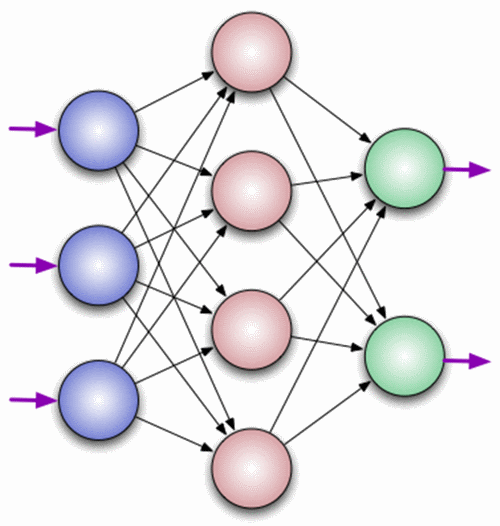
\includegraphics[width=0.7\linewidth]{images/nn.png}
	\caption{Sieć neuronowa typu propagation.}
	\label{fig:nn}
\end{figure} 

W tym przypadku stosowanie sieci o bardziej złożonych strukturach wydaje się zbędny i sprzeczny z intuicją. Sieci te doskonale rozpoznają cechy wartości podanych na wejście co powoduje poprawne zachowanie dla sygnałów zbliżonych z którymi sieć nie miała wcześniej styczności. 

Również ważną cechą sieci jest dobór funkcja przejścia dla neuronów. W tym przypadku została zastosowana funkcja $tanh(x)$ ze względu na jej charakterystykę, która akcentuje wartości brzegowe, które w naszym przypadku odpowiadają wykryciu skóry przez sieć. 

Po implementacji sieci przystąpiono do adaptacji algorytmu uczenia. W sieciach typu propagation najczęsciej stosowany jest algorytm backpropagation, który cechuje się prostą lecz również długim czasem uczenia sieci oraz żmudnymi obliczeniami. Polega on na podawaniu na wejście sieci wektor odpowiednich wartości, a następnie wyznaczaniu różnicy wyjścia sieci z wartością oczekiwaną. Różnica ta jest przetwarzana wstecznie przez sieć wraz z wyznaczaniem gradientów błędów poszczególnych neuronów. Na ich podstawie korygowane są wagi każdego z wejść neuronów co powoduje uczenie sieci.

Wszystkie skrypty utworzone na tym etapie oraz obszerna baza danych umożliwiły rozpoczęcie prac nad uczeniem sieci. Wywołanie odpowiednich skryptów rozpoczynało proces uczenia sieci, którego czas trwania zależał od ilości wykonania powyżej opisanej operacji dla każdego z wierszy. Optymalne wyniki otrzymane były dla około 100 iteracji. Warto również wspomnieć, iż początkowo baza zawierała dane posortowane ze względu na wektor oczekiwanego wyjścia co zdecydowanie utrudniało proces uczeni. Rozwiązano ten problem przez przemieszanie wierszy w bazie.

Na rysunku \ref{fig:reka} przedstawiono przykładowe przetworzenie małego obrazka na którym testowano sieć po zakończeniu uczenia. Na jego podstawie wstępnie oceniano powodzenie procesu uczenia sieci. Jak widać na rysunku udało się osiągnąć zadowalającą jakość. Warto zauważyć, iż zdjęcie testowe zostało wykonane przez autorów projektu więc wartości RGB poszczególnych pikseli są niezależne względem tych umieszczonych w bazie.

\begin{figure}[tbph!]
	\centering
	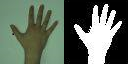
\includegraphics[width=0.6\linewidth]{images/reka.png}
	\caption{Przykładowy wynik testu działania sieci po uczeniu.}
	\label{fig:reka}
\end{figure}

W kolejnej fazie zmodyfikowano system reprezentacji liczb na których bazuje działanie sieci neuronowych. Zastosowano zmienne typu fixed\_point, które pozwalają na dokładne określenie ilości bitów przeznaczonych na reprezentacje poszczególnej liczby. Do konwersji z typu double do typu fixed\_point został stworzona funkcja w środowisku MATLAB. Jako argument przyjmuje ona zmienną typu double, a następnie na podstawie sztywno określonej konfiguracji funkcji tworzy zmienną typu fixed\_point, która reprezentuje wartość argumentu lub wartość najbliższą, która jest możliwa do zaprezentowania. Zabieg ten miał na celu dokładne odwzorowanie działania sieci na układzie fpga. Czas przetwarzania obrazu testowego przez sieć, a w szczególności sam proces uczenia wydłużył się kilkakrotnie ze względu na liczne konwersje.

Po przeprowadzaniu ponownego procesu uczenia oraz sprawdzeniu, że modyfikacje te nie zaburzyły w znaczny sposób działania sieci zakończono proces tworzenia odwzorowania sieci w środowisku MATLAB. 

Podczas realizacji tej fazy zorientowano się, iż właściwa implementacja na układzie fpga nie wymaga implementowania procesu uczenia w znacznym stopniu upraszcza implementacje. Uzyskane dotychczas informacje na temat topologii sieci, funkcji przejścia, wartości poszczególnych wag dla każdego z neuronów oraz optymalnej ilości bitów przeznaczonych do reprezentacji tych wartości pozwoliły na przystąpienie do ostatniego etapu.

\section{Realizacja algorytmu w środowisku ISE}



\chapter{Efekt działania}
\label{cha:efekt}



%----------------------------------------------------------------------------------------
% Rozbudować
% - tu są tylko główne myśli
% - 
%----------------------------------------------------------------------------------------
\section{Efekt działania}
W tym rozdziale zostały zebrane zdjęcia zrobione podczas testowania algorytmu. Niestety z powodu braku odpowiedniego sprzętu zdjęcia te zostały zrobione w słabej jakości. Warto zauważyć, że w bazie znajdowały się również wartości RGB dla ludzi o różnej karnacji. Skutkuje to tym, iż na zdjęciu \ref{fig:5} sieć bez problemu rozpoznaje również skórę innej karnacji.\\ \\ 
\begin{figure}[tbph!]
\centering
\includegraphics[width=0.9\linewidth]{images/1.png}
\caption{Dłoń na tle pracowni.}
\label{fig:1}
\end{figure}
\begin{figure}[tbph!]
\centering
\includegraphics[width=0.9\linewidth]{images/3.png}
\caption{Osoba w koszulce na tle pracowni.}
\label{fig:2}
\end{figure}
\begin{figure}[tbph!]
\centering
\includegraphics[width=0.9\linewidth]{images/2.png}
\caption{Dłoń na tle szafy.}
\label{fig:3}
\end{figure}
\begin{figure}[tbph!]
\centering
\includegraphics[width=0.9\linewidth]{images/5.png}
\caption{Szerszy widok na pracownie.}
\label{fig:4}
\end{figure}
\begin{figure}[tbph!]
\centering
\includegraphics[width=0.9\linewidth]{images/4.png}
\caption{Rozpoznanie skóry osoby innej rasy.}
\label{fig:5}
\end{figure}

\chapter{Podsumowanie}
\label{cha:podsumowanie}

\section{Wnioski}
Udało się zrealizować wszystkie założenia projektu. Nie mniej jednak warto mieć na uwadze, iż udało się udowodnić jedynie poprawność działania algorytmów opartych na sieciach neuronowych. Jakość obrazu oraz dokładność rozpoznawania może zostać poprawiona przy użyciu filtrów medianowych oraz nie wyklucza się, iż zmiana topologii może spowodować lepsze rezultaty. Zmiany te powinny zostać wprowadzone w pierwszym etapie dalszych prac nad projektem. Z powodu nie wystarczającej ilości czasu kolejne prace nad udoskonaleniem algorytmu nie zostały zrealizowane.
\chapter{Dodatek}
\label{cha:dodatek}

\section{Opis plików}
Wszystkie pliki utworzone podczas pracy nad projektem zostały wysłane razem ze sprawozdaniem oraz są dostępne pod adresem \url{http://github.com/Kyhu/wsw-neuro}, gdzie mogą być w dalszym ciągu aktualizowane. Poniżej krótko opisano strukturę projektu.

\begin{figure}[tbph!]
\centering
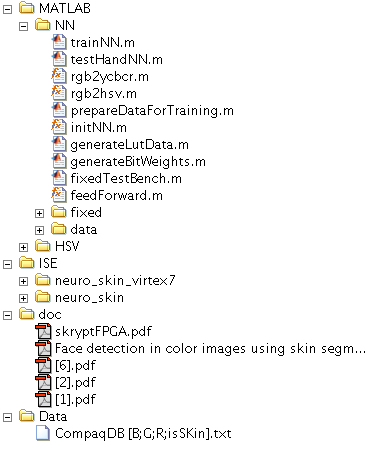
\includegraphics[width=0.63\linewidth]{images/tree.png}
\caption{Struktura katalogów}
\label{fig:tree}
\end{figure}

\begin{itemize}
\item MATLAB - folder zawierający wszystkie utworzone pliki środowiska MATLAB.
\subitem NN
\subsubitem trainNN.m - skrypt trenujący model sieci neuronowej.
\subsubitem testHandNN.m - skrypt testujący sieć na przykładowym obrazie.
\subsubitem generateLutData.m - skrypt generujący dane dla LUTa w module języka verilog.
\subsubitem generateBitWeights.m - skrypt generujący linijki kodu veriloga odpowiadające za przechowywanie wartości wag sieci neuronowych.
\subsubitem fixedTestBench - test bench dla skryptów feedForward oraz fix\_feedforward.
\subsubitem feedForward.m - funkcja symulująca moduł neural\_networks.v na liczbach zmiennoprzecinkowych
\subsubitem fix\_feedForward.m - funkcja symulująca moduł neura\_networks.v na liczbach stałoprzecinkowych
\subsubitem data - folder zawierający zapisane modele sieci Neuronowych (wagi) oraz testowe obrazy.
\subitem HSV - folder zawierający skrypty wykorzystane do testowania modułu rgb2hsv zaimplementowanego w veriolgu.
\item ISE - folder zawierający projekty realizowane w środowisku ISE.
\subitem neuro\_skin - projekt finalny realizowany na kartę Spartan-6.
\subitem neuro\_skin\_virtex7 - projekt finalny przerzucony na tor wizyjny karty virtex7 (z projektu pbas)
\item doc - folder zawierający wykorzystane artykuły naukowe. Artykuł dostarczony przez prowadzącego jest opisany pełnym tytułem, pozostałe są oznaczone odnosząc się do jego bibliografii.
\item Data - folder zawierający bazę danych wykorzystaną do trenowania sieci neuronowej. (Compaq Database - \url{https://archive.ics.uci.edu/ml/machine-learning-databases/00229/Skin_NonSkin.txt})
\end{itemize}


%----------------------------------------------------------------------------------------
%	BIBLIOGRAPHY
%----------------------------------------------------------------------------------------

\bibliographystyle{plain}
\bibliography{bibliography}
%\addcontentsline{toc}{chapter}{\textcolor{ocre}{Bibliography}}
%\section*{Books}
%\addcontentsline{toc}{section}{Books}
%\printbibliography[heading=bibempty,type=book]
%\section*{Articles}
%\addcontentsline{toc}{section}{Articles}
%\printbibliography

%----------------------------------------------------------------------------------------
%	INDEX
%----------------------------------------------------------------------------------------

%\cleardoublepage
%\setlength{\columnsep}{0.75cm}
%\addcontentsline{toc}{chapter}{\textcolor{ocre}{Index}}
%\printindex

%----------------------------------------------------------------------------------------

\end{document}